
\section{Data}

\subsection{Natural Disaster Data}

Natural disasters are declared as such by the president, usually upon request by the affected state's governor. Once a disaster is federally declared, states or local governments can receive federal assistance. The Federal Emergency Management Agency (FEMA) provides data on all federally declared natural disasters, beginning in 1953. The data is easily accessible via their API \citep{rfema}.



Figure \ref{DisasterMap} shows the number of declared disasters since 1953 across the US.


\begin{figure}[!h]
	\centering
	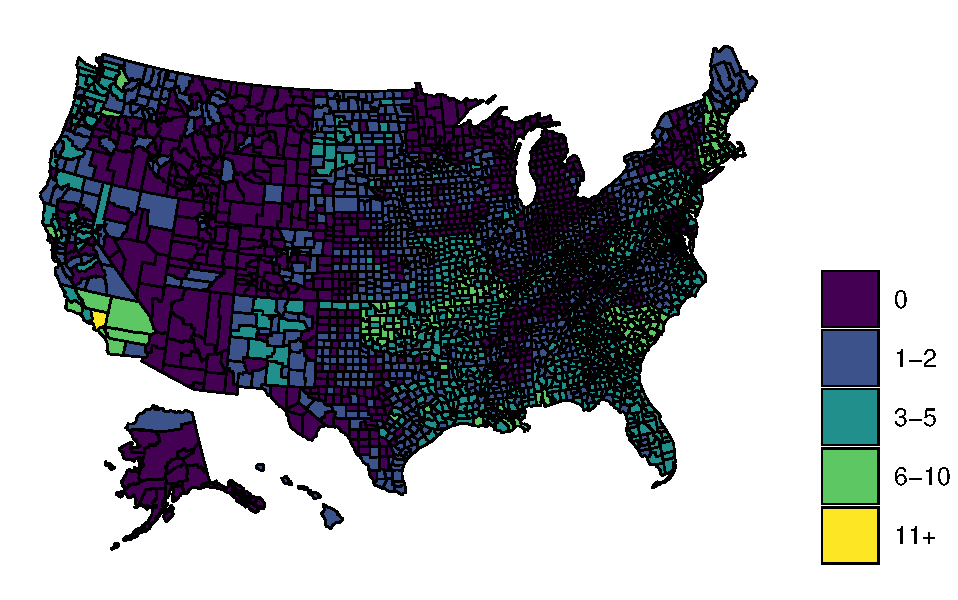
\includegraphics[scale=0.7]{"../Code & Data/DisasterMap.png"}
	\caption{Number of declared natural disasters by county}
	\label{DisasterMap}
\end{figure}



\subsection{Standardized Testing Data}

Data on academic achievement is available from the Stanford Education Data Archive \citep{SEDA}. They provide mean test results from standardized tests by county, year, grade and subject among all students and various subgroups (including race, gender, and economicall disadvantaged). The most recent version 4.1 covers grades 3 through 8 in mathematics and Reading Language Arts (RLA) over the 2008-09 through 2017-18 school years.

Test scores are cohort-standardized, meaning they can be interpreted relatively to an average national reference cohort in the same grade. For instance, a county mean of 0.5 indicates that the average student in the county scored approximately one half of a standard deviation higher than the average national student in the same grade.

Figure \ref{TestScoresMap} shows the average test scores across the US.


\begin{figure}[!h]
	\centering
	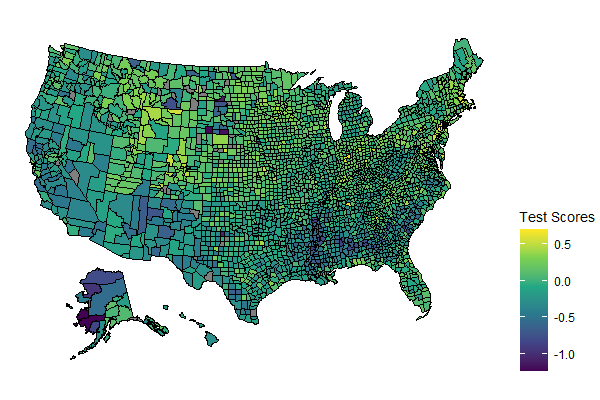
\includegraphics[scale=0.7]{"../Code & Data/TestScoresMap.png"}
	\caption{Average test scores by county (cohort-standardized and averaged across grades, subjects and years)}
	\label{TestScoresMap}
\end{figure}

Natural disasters should only have an effect on test scores if they occur before the test. Standardized tests are generally administered during spring. We will use March 1st as a cut-off point. Thus, any disaster happening within the same school year before the 1st of March will be considered. School years tend to start in late August or early September with some variation across states. We will use September 1st, meaning any disaster happening between September 1st and March 1st will be counted for a given school year.







